\documentclass[9pt,twocolumn,twoside]{styles/osajnl}
\usepackage{fancyvrb}
\usepackage[colorinlistoftodos,prependcaption,textsize=normal]{todonotes}
\newcommand{\TODO}[2][]{\todo[color=red!10,inline,#1]{#2}}
\newcommand{\GE}{\TODO{Grammar}}
\newcommand{\SE}{\TODO{Spelling}}
\newcommand{\TE}{\TODO{Term}}
\newcommand{\CE}{\TODO{Citation}}

\journal{i524} 

\title{Apache Lucene}

\author[1,*, +]{Roy Choudhury, Sabyasachi}

\affil[1]{School of Informatics and Computing, Bloomington, IN 47408, U.S.A.}

\affil[*]{Corresponding authors: sabyroyc@indiana.edu}

\affil[+]{HID - S17-IO-3015}

\dates{project-000, \today}

\ociscodes{Search Engine Library, Lucene}

% replace this with your url in github/gitlab
\doi{\url{https://github.com/sabyasachi087/sp17-i524/tree/master/paper1/S17-IO-3015/report.pdf}}


\begin{abstract}
This paper gives an overview of Apache Lucene. We will go through the basic architecture and functionality of the library. We will see the advantages and downfalls of Lucene and conclude on its implementation.
\newline
\end{abstract}

\setboolean{displaycopyright}{true}

\begin{document}

\maketitle

\TODO{This review document is provided for you to achieve your
  best. We have listed a number of obvious opportunities for
  improvement. When improving it, please keep this copy untouched and
  instead focus on improving report.tex. The review does not include
  all possible improvement suggestions and for each comment you may
  want to check if it applies elsewhere in the document.}

\TODO{Abstract: Please redo. The abstract needs to be about the
  technology, not about the paper itself. You should say briefly what
  the most important things about Lucene are. Then maybe in the last
  sentence, you can tell the reader what the paper will cover. This is
  the part of the paper that the most people will read, and will use
  it to decide whether to read on. As it stands, someone reading your
  abstract will still have no idea what Lucene is if they didn't
  before.}

\TODO{Please, format lines to 80 characters in the source to make the
  LaTeX easier to read.}

\TODO{You need to expand your paper. Currently, it's closer to one
  page, excluding diagram and references. It needs to be two pages.}

\TODO{Overall, your paper needs to be more detailed when describing
  specific functions. In several places you use very general sentences
  that don't provide information, and someone would have to already
  know about search engines and Lucene to evaluate them. Please see
  the comments below for details.}

\TODO{Assessment: Revisions required. Please address the review
  comments by end of March.}

\section{Introduction}

Apache Lucene is a search library that enables search facility to any
application. Although it was initially written in Java but has been
\GE ported to many languages chiefly C-Sharp, c/c++ \GE, Python
etc. It is an active open source project and under Apache License. Its
latest release is
\href{http://lucene.apache.org/core/6_4_1/index.html}{6.4.1}. \TODO{The
  version is out of scope for the paper. The paper should be able to
  stand more generally, independent of when it was written. If you
  think it's really important to mention the version (e.g. there are
  significant changes after a given version, you can state that in a
  footnote. That way you won't break up the flow of the paper with
  information that most readers won't care about.} It is important
that we must understand that \TODO{The beginning of this sentence is
  unnecessary. Try to keep your sentences shorter and to the point; it
  will make reading the paper easier.} Lucene is just a search library
and cannot handle other related stuffs like crawling, document
filtering , administration etc.

\section{Concepts}
To understand the purpose of Lucene we have to be familiar with two
terms, one is "Information Overload" and "Information
Retrieval"\cite{wiki-ir} \TODO{Leave a space between the referece and
  the previous word.}.  \TODO{When you introduce terms, if you want to
  draw attention to them, it's better to use the LaTeX \\emph\{\}
  command, rather than quotes.}  \TODO{Like before, you should try to
  get straight to the point. This first sentence doesn't help the
  reader understand anything about Lucene, IR or information overload,
  so it can be skipped. You can start by describing information
  overload like you do later in this paragraph.} The term information
overload means, difficulty that one can have in making decisions,
because of the presence of too much of information. In another \TE
words, "Information Overload" \TODO{You've already introduced the term
  so no need for quotes or special formatting anymore.} can occur if
the rate of feed/input into a system exceeds its processing
capabilities. Imagine the situation of current world. We are living in
the world where data has reached volume of zeta bytes. To extract some
insight , first step is to collect all related data. This is known as
information retrieval(IR). IR is the task of collecting relevant
information from collection of data resources scattered across
devices. Now with the above understanding we can say Lucene is a
scalable Information Retrieval library.

\subsection{Lucene and Search Engine}
Google has set some base expectations for search engines, which if not
available can cause dissatisfaction for the users. For example spell
checker and response time of <= 1 second. Lucene should be able to met
those expectations or else its \TE \TODO{Know when to use "it is"
  versus "its"} not worth. \GE But \TODO{Avoid starting a sentence
  with "and", "but", "so".} Lucene is not a full fledged search engine
rather its a tool kit to achieve so. \GE So \TE lets jot down the
steps for any search engine \TODO{"jot down" is too conversational for
  a paper like this.}

Module  : Raw Content -> Gather Data -> Analyze -> Index ->  Query Support 
UseCase : User query -> Search Engine -> Build Query -> Extract Information from indexed data

\TODO{This can be expanded significantly. It basically describes what a search engine does, but provides almost no detail. If someone reading this doesn't already know how search engines work, they won't be helpful.}

\section{Architecture}
Figure 1 explains a basic architecture of Lucene

\begin{figure}[htbp]
\centering
\fbox{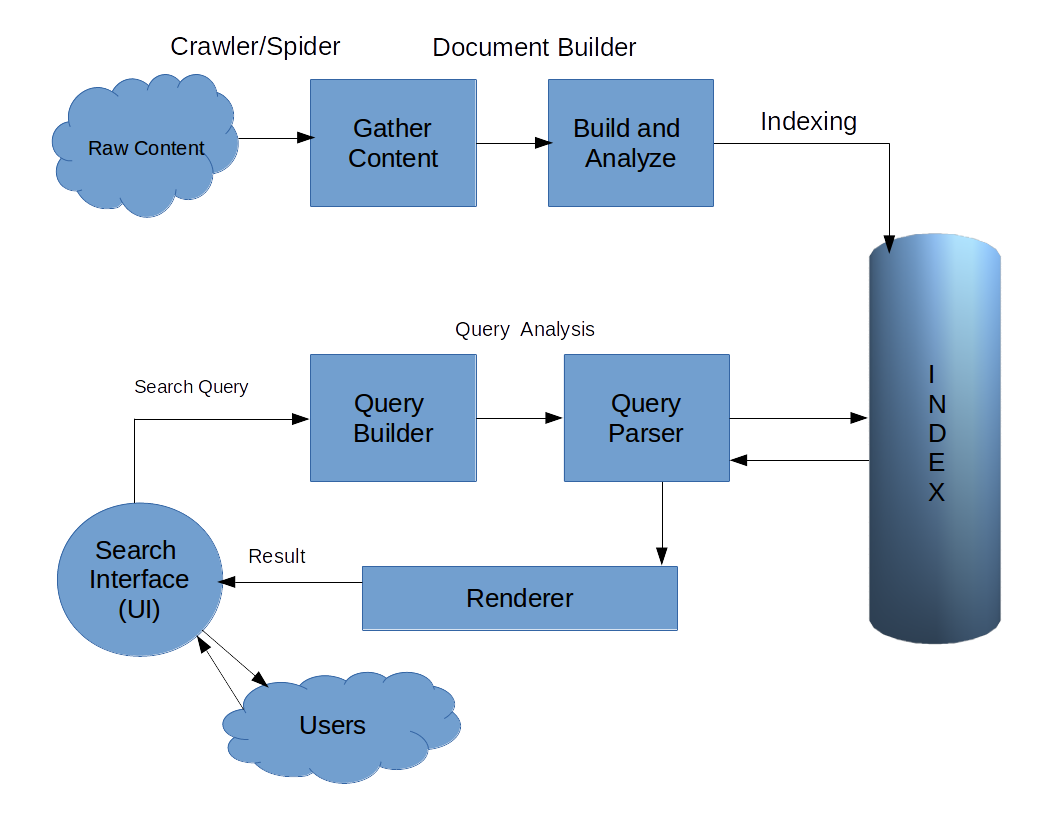
\includegraphics[width=\linewidth]{images/Apache_Lucene_Architecure.png}}
\caption{Apache Lucene Architecture.} \TODO{Did you create this
  diagram? If not, you need to add a reference to where you got it
  from.}
\label{fig:lucene-data-flow}
\end{figure}

Lucene library is compact and does not have any external
dependencies. But \TE it can be plugged \TE with other libraries for
building a search engine. \TODO{What other libraries? You've already
  said Lucene doesn't provide everything needed for a search engine,
  so you need to explain exactly what it provides, and what other
  technologies someone working on a search engine will need. Imagine
  you are a user who wants to set up a search engine for their
  data. Other than Lucene, what else will they need?} Fig
1\cite{lucene-book} shows process flow of Lucene. \GE On a high level
, data collected from different sources are analyzed and converted
into smaller chunks. These are known as documents. Documents are text
entries and from these text entries Lucene performs indexing and store
it in local disk for future reference. \TODO{What is the purpose of
  indexing?} The next step is to handle the search query from
users. Lucene has a query parser to understand the query and search
the index for the correct or relevant match. If found, returns the
document back. We will elaborate the flow beneath.

\section{Lucene Components}

\subsection{Document Analysis and Indexing}
Data or contents which are available in different format and location
needs to be gathered. This process is typically done by a
crawler/spider. Core Lucene does not have these capabilities and can
be considered to be a pre-requisite for Lucene to
implement. \TODO{It's important to mention that Lucene can be made to
  work on any document collection or database. You don't need to crawl
  anything from the Internet.} Two of the crawler that are build on
Lucene are \href{http://lucene.apache.org/solr}{Solr} and
\href{http://lucene.apache.org/nutch}{Nutch}.  \TODO{These need to be
  added as references in references.bib, not simply as links.}  Once
the data is collected , document has to be constructed from the
contents. The design of constructing documents has to be decided by
the user and implemented within Lucene. Lucene provides an API for
building documents but logic has to be provided by the implementation
layer. Lucene also does not provide any API for document
filtering. \TODO{What is document filtering? How does it fit into the
  basic process of collecting the data, preprocesssing it for Lucene,
  and Lucene indexing it?} But yet again we have Tika , which is built
on Lucene, can be used for this purpose. But we cannot index the
document yet. \TODO{This and the next sentence say the same
  thing. Redundancy.} We cannot index the raw content within the
document directly. Before that , we need to break the content into
smaller chunks known as tokens. Each token is map to a
"word". \TODO{Not clear what this sentence says. Is a token a word?
  Why is "word" quoted?} Analysis includes handling compound words,
spell check, typo correction injection of synonyms, etc. Lucene has
built in support of list of analyzers \GE \TODO{Where do these
  analyzers fit in the Lucene architecture?} which gives a fine grain
control over analysis. Once tokenization is done , now \TE its
\TODO{"it is"} time for indexing. Lucene takes care all of the need to
cater this step. An API has been provide for this purpose, but has to
be implemented carefully as the searching will solely depend upon how
well the indexing has been done. \TODO{You need to explain what
  exactly indexing is. This portion is a bit too general and is not
  clear if you don't already know what indexing is.}


\subsection{Searching}
It is a look up process \TODO{Need a full sentence, don't refer to the
  section title. "Searching is the process of looking up..."} within
the index to extract the most relevant (matching) documents. It is
based on two matrices \TODO{Do you mean metrics?} i.e. \TE Precision
and Recall. Recall measures how well the system finds the relevant
documents and Precision measures the filtering out the irrelevant
one. \TODO{Not a good explanation of precision and recall. Recall
  measures the fraction of relevant documents that are
  retrieved. Precision measures the fraction of retrieved documents
  that are relevant.} Lucene offers benchmarking technique for
measuring these matrices \TE. User Interface (UI) is equally important
for a search application as that is what the end user is going to
use. Lucene does not provide any UI support. When user inputs the
search query the first step is to build the query. User inputs are
human readable and need further processing before it can be used
within the application. Lucene provides a powerful parser for this job
known as QueryParser. Even it is default state \GE it does the job
pretty clean \TODO{"pretty clean" is too vague.} but often needs
extension as per some advance requirements. Finally hitting the search
query to index. \TODO{This is not a complete sentence.} Almost
everything about this is catered by Lucene and also provide option for
extension. \TODO{"Almost everything about this is catered by Lucene"
  is too general; it doesn't provide any useful information} It finds
the result and returns all relevant document objects. Its \TODO{"it is"} the
responsibility of the UI to render the results correctly.

\section{Advance Usages} \TE
Lucene has some advance feature for administration and analytics. For
example Lucene allows to configure the RAM buffer size , re-indexing
,commit and purge scheduler. \TODO{You need to provide a little more
  detail what these things are.} It allows some fault tolerance
mechanism in case a newly added document failed to index. Related to
analytics it also provides some meta information regarding the search
queries it receives and the results it renders. For example which kind
of query are run , query hitting lowest relevance , query having no
results and so on. One big problem within the list of advance usages
\TE that Lucene does not support is "Scaling" \TODO{Don't use
  quotes.}. Scaling in terms of both through put and processing
speed. In a clustered environment this is quiet \TE an important part
as data and resource all are distributed. But both Solr and Nutch
provides data partitioning and sharding to achieve higher throughput
if not speed. Elastic search \TODO{What is elastic search? You either
  need to explain briefly or provide a reference.} is another option
which is based upon Lucene and provides distributed computing.


\section{Conclusion}
Lucene is the standard library for search applications. It can be
compared with 'C' (language) of computing which is small and powerful
but requires much more \TE effort to build an entire
application. \TODO{The comparison is a stretch, and subjective.} It
must be remembered that Lucene is just a library which sits at the
core of the functionality but it needs much more \TODO{"much more" to
  vague; avoid using adjectives like "much" in a paper like this.}
than that to build an application. Elastic Search , Solr and Nutch
which are based on Lucene are preferred tools in terms of building
enterprise level search engines.

\section{Reading Sources}

\begin{itemize}
\item Lucene In Action \cite{lucene-book} provides a startup guide to
learn, build and implement search engines based on Lucene 
\item Lucene at tutorial point \cite{www-lucene-tp} provides introduction
 to Lucene Library.
\end{itemize}



\section*{Acknowledgements}

Thanking Prof. Gregor von Laszewski for his technical help and support.


% Bibliography

\bibliography{references}

\end{document}
